\documentclass{bioinfo}
\copyrightyear{2005}
\pubyear{2005}

\begin{document}
\firstpage{1}

\title[Sparse SVD incorporating stability selection]{Robust biclustering by sparse singular value decomposition incorporating stability selection}
\author[Sill \textit{et~al}]{Martin Sill\,$^{1,\footnote{to whom correspondence should be addressed}}$, Sebastian Kaiser\,$^{2}$, Axel Benner\,$^{1}$\\
and Annette Kopp-Schneider\,$^{1}$

}
\address{
$^{1}$Division of Biostatistics, German Cancer Research Center, 69120 Heidelberg, Germany \\
$^{2}$Working Group Computational Statistics, LMU-M\"unchen, 80539 M\"unchen, Germany\\
}
\history{Received on XXXXX; revised on XXXXX; accepted on XXXXX}

\editor{Associate Editor: XXXXXXX}

\maketitle

\begin{abstract}
\section{Motivation:} 
Over the past decade several biclustering approaches have been published in the field of gene expression data analysis.
Despite of huge diversity regarding the mathematical concepts of the different biclustering methods, many of them can be related to the singular value decomposition (SVD). Recently, a sparse SVD approach (SSVD) has been proposed to reveal biclusters in gene expression data. In this article, we propose to incorporate stability selection to improve this method. Stability selection is a subsampling based variable selection that allows to control Type I error rates. The here proposed S4VD algorithm incorporates this subsampling approach to find stable biclusters and to estimate the selection probabilities of genes and samples to belong to the biclusters. 
\section{Results:}
\textcolor{red}{So far, the S4VD method is the first biclustering approach that takes the cluster stability regarding perturbations of the data into account.
Application of the S4VD algorithm to a lung cancer microarray data set revealed biclusters that correspond to coregulated genes associated with cancer subtypes. Marker genes for different lung cancer subtypes showed high selection probabilities to belong to the corresponding biclusters. Moreover, the genes associated with the biclusters belong to significantly enriched cancer related Gene Ontology categories. In a simulation study the S4VD algorithm outperformed the SSVD algorithm 
and two other SVD related biclustering methods in recovering artificial biclusters and in being robust to noisy data.}
\section{Availability:}
R-Code of the S4VD algorithm as well as a documentation can be found at \href{http://s4vd.r-forge.r-project.org/}{http://s4vd.r-forge.r-project.org/}.
\section{Contact:} \href{m.sill@dkfz.de}{m.sill@dkfz.de}
\section{Supplementary information:} Supplementary data are available at
\textit{Bioinformatics} online.
\end{abstract}

\section{Introduction}
Clustering methods belong to the most commonly used statistical tools in the analysis of high dimensional data sets. If additional information about the sample class labels is lacking, other types of analysis like supervised classification methods or testing for differentially expressed genes can not be performed. In this case unsupervised clustering allows to reveal unknown structures that are possibly hidden in the gene expression data matrix. These structures may be characterized by groups of genes that are coregulated by a common transcription factor and thus belong to the same pathway or samples that share a similar gene expression pattern. 

%Classical clustering methods are hierarchical clustering or k-means clustering. 
One disadvantage of commonly used clustering algorithms like hierarchical clustering or k-means clustering is that the cluster assignment of objects are based on the complete feature space, e.g. in case of clustering the samples the resulting clusters are derived with respect to all genes. 
But groups of genes may only be coregulated within a subset of the samples and samples may share a common gene expression pattern only for a subset of genes. Such clusters that exist only in a subspace of the feature space can hardly be detected by these classical one-way clustering algorithms.
To find such clusters other clustering concepts are needed. 

In the past decade, the concept of biclustering has emerged in the field of gene expression analysis. Biclustering which is also known as coclustering or two-way clustering describes the simultaneous clustering of the rows and the columns of a data matrix. 
The first biclustering algorithm, the so called Block Clustering, has been developed by Hartigan (1972)\nocite{Hartigan1972}. 
Cheng and Church (2000)\nocite{Cheng2000} proposed the first biclustering algorithm for the analysis of high dimensional gene expression data.
Since then, many different biclustering algorithms have been developed. 
Currently, \textcolor{red}{there} exists a diverse spectrum of biclustering tools that follow different strategies and algorithmic concepts.
Among others, popular algorithms are the Coupled Two-Way Clustering (CTWC) by Getz et al. (2000) 
\nocite{Getz2000}, Order Preserving Sub Matrix (OPSM) algorithm by Ben-Dor et al. (2003)\nocite{BenDor2003}, %FLOC by Yang et al. (2003)\nocite{Yang2003}, Spectral biclustering by Kluger et al. (2003)\nocite{Kluger2003}, %xMotif by Murali and Kasif (2003)\nocite{Kasif2003},
the Iterative Signature Algorithm (ISA) by Bergmann et al. (2003)\nocite{Bergmann2003},
the Plaid Model by Lazzeroni and Owen (2002)\nocite{Lazzeroni2000} and the improved Plaid Model (Turner et al., 2005)\nocite{Turner2005}, SAMBA by Tanay et al. (2004)\nocite{Tanay2004}, biclustering by non-smooth non-negative matrix factorization by Carmona-Saez et al. (2006)\nocite{Carmona-Saez2006}, the Bi-correlation clustering algorithm (BCCA) by Bhattacharya and De (2009)\nocite{Bhattacharya2009} and factor analysis for bicluster acquisition (FABIA; Hochreiter et al., 2010)\nocite{Hochreiter2010}. Prelic et al. (2006)\nocite{Prelic2006} developed a fast divide-and-conquer algorithm (Bimax) and conducted a systematic comparison of different biclustering algorithms.
Santamaria et al. (2007)\nocite{Santamaria2007} published an article on validation indices for the evaluation of biclustering results and the comparison for biclustering algorithms. Comprehensive reviews about the concept of biclustering and the different biclustering approaches have been written by Madeira and Oliveira (2004)\nocite{Madeira2004} and Van Mechelen et al. (2004)\nocite{Mechelen2004}.

In a more theoretical review Busygin et al. (2008)\nocite{Busygin2008} emphasized the mathematical concepts behind several biclustering algorithms and pointed out that the SVD represents a capable tool for finding biclusters. Furthermore, most existing biclustering algorithms use the SVD directly or have a strong association with it. To keep track of the huge diversity, regarding the mathematical properties of the existing biclustering algorithms, Busygin et al. (2008) suggest to relate new and existing biclustering algorithms to the SVD. 

A major drawback of many biclustering methods is that they rely on random starting seeds and thus are inconsistent and results may vary even when the algorithm is applied to the same data set. As often in unsupervised clustering it is difficult to judge the biclustering results regarding their stability. For one-way clustering several resampling approaches to validate the stability of the clustering results are known, e.g. %bootstrap clustering (Kerr and Churchill, 2001)\nocite{Kerr2001},
multiscale bootstrap hierarchical clustering (Suzuki and Shimodeira, 2006)\nocite{Suzuki2006} and consensus clustering (Monti, 2005)\nocite{Monti2003}. In case of biclustering, similar methods that take the stability of the results into account are not yet available. 

Recently, Lee et al. (2010)\nocite{Lee2010} proposed a sparse SVD (SSVD) method to find biclusters in gene expression data. Singular vectors of an SVD are interpreted as regression coefficients of a linear regression model. The SSVD algorithm alternately fits penalized regression models to the singular vector pair to obtain a sparse matrix decomposition. The sparseness of the resulting singular vectors strongly depends on the choice of the penalization parameter. In this article, we propose to choose the penalization parameters by stability selection (Meinshausen and B\"uhlmann, 2010)\nocite{Meinshausen2010} which is a subsampling procedure that can be applied to penalized regression models to select stable variables. In addition, stability selection offers the possibility to control Type I error rates (Dudoit et al., 2003)\nocite{Dudoit2003}, e.g. the per-family error rate (PFER) or the per-comparison wise error rate (PCER). 
Applying the new combined algorithm, the sparse SVD algorithm with nested stability selection (S4VD), to a lung cancer gene expression data set reveals biclusters that represent lung cancer subtypes characterized by relevant sets of coregulated genes. In a simulation study we compare the S4VD with the SSVD algorithm as well as the improved Plaid Model (Turner et al., 2005) and the ISA (Bergmann et al., 2003).
\vspace{- .15 cm}
\begin{methods}
\section{Methods}
\subsection{SVD and Biclustering}
Let $\mathbf{X}=(x_{ij}) \in \mathbb{R}^{p \times n}$  be the gene expression matrix with indices $i=1,\cdots,p$ and $j=1,\cdots,n$. The number of genes $p$ is usually by multiple greater than the number of samples $n$. The SVD of $\mathbf{X}$ can be written as:
\begin{equation}
 \mathbf{X} \approx \mathbf{U}\mathbf{D}\mathbf{V}^{T} = \sum_{k=1}^{r}d_{k}\mathbf{u}_{k}\mathbf{v}_{k}^{T},
\end{equation}
where $r$ is the rank of $\mathbf{X}$ and the columns of the matrix $\mathbf{U}=(\mathbf{u}_{1},\cdots,\mathbf{u}_{r})$ are the orthonormal left-singular vectors  and the columns of $\mathbf{V}=(\mathbf{v}_{1},\cdots,\mathbf{v}_{r})$ are the orthonormal right-singular vectors. The elements of the diagonal matrix $\mathbf{D}$ are the corresponding positive singular values $d_{1} \geq d_{2} \geq \cdots d_{r} > 0$. 
Thus the SVD is the sum of rank one matrices $d_{k}\mathbf{u}_{k}\mathbf{v}_{k}^{T}$, herein after also called SVD-layers.
According to Busygen et al. (2008) biclustering can be related to the SVD by considering an idealized data matrix.
This matrix has a block diagonal structure where each block represents a bicluster and the elements outside these blocks are equal to zero:
\begin{equation}
\mathbf{X}=
\begin{pmatrix} 
\mathbf{X}_{1} & 0 & \cdots & 0\\
0 & \mathbf{X}_{2} & 0 & \cdots \\
\vdots  & \vdots  & \ddots  & 0 \\
0 & 0 & \cdots & \mathbf{X}_{r}
\end{pmatrix},
\end{equation}
where $\mathbf{X}_{k}$, $k=1,\cdots,r$ are submatrices of $\mathbf{X}$. If we decompose $\mathbf{X}$ by the SVD, then each submatrix $\mathbf{X}_{k}$ will be associated with a singular vector pair $(\mathbf{u}_{k},\mathbf{v}_{k})$ such that the non-zero coefficients in $\mathbf{u}_{k}$ represent the rows that belong to $\mathbf{X}_{k}$ and the non-zero coefficients $\mathbf{v}_{k}$ represent the columns that belong to $\mathbf{X}_{k}$. In the presence of noise and if the data matrix has no block diagonal structure, the SVD will still be able to detect the rows and columns of the submatrices as the prominent coefficients in the singular vector pair. These properties make the SVD a practical method for biclustering. 

\subsection{The SSVD Algorithm}
A sparse SVD method for biclustering high-dimensional gene expression data has been proposed by Lee et al. (2010). The idea is to interpret the singular vectors of a regular SVD as regression coefficients of a linear regression and use sparsity-inducing penalties to obtain sparse singular vector pairs.\\
According to Eckart and Young (1936)\nocite{Eckart1936} the first SVD-layer gives us the best rank-one approximation of $\mathbf{X}$ with respect to the squared Frobenius norm, i.e. 
\begin{equation}
 (d_{1},\mathbf{u}_{1},\mathbf{v}_{1})=\text{arg} \mathop{\mbox{min}}_{d,\mathbf{u},\mathbf{v}} \left\Vert \mathbf{X} - d\mathbf{u}\mathbf{v}^{T} \right\Vert_{F}^{2},
\label{eq:3}
\end{equation}
where $\left\Vert \cdot \right\Vert_{F}^{2}$ indicates the squared Frobenius norm, which is the sum of squared elements of the matrix.
Lee et al. (2010) showed how this rank-one approximation can be related to linear regression. Suppose $\mathbf{u}_1$ is fixed, then the minimization of (\ref{eq:3}) with respect to $(d_{1},\mathbf{v}_{1})$ is equivalent to a minimization with respect to  $\mathbf{\tilde{v}}_{1}=(d_{1}\mathbf{v}_{1})$.
Accordingly, the loss function can be written as minimization of the squared $\textit{l}^{2}$-norm:
\begin{equation}\left\Vert \mathbf{X} - \mathbf{u}_{1}\mathbf{\tilde{v}}_{1}^{T}\right\Vert_{F}^{2}=
\left\Vert \mathbf{y}-(I_{n}\otimes\mathbf{u}_{1})\mathbf{\tilde{v}}_{1}\right\Vert,
\label{eq:4}
\end{equation}
where $\mathbf{y}=(\mathbf{x}_{1}^{T},\cdots,\mathbf{x}_{n}^{T})^T \in \mathbb{R}^{pn}$ with $\mathbf{x}_{j}$ being the $j$th column of $\mathbf{X}$. Then the minimization of (\ref{eq:4}) can be interpreted as least squares problem with $\mathbf{y}$ as the response vector, $I_{n}\otimes\mathbf{u}_{1}$ as the design matrix and the $\mathbf{\tilde{v}}_{1}$ as vector of regression coefficients. The least squares estimator of $\mathbf{\tilde{v}}_{1}$ is: 
\begin{equation}
\begin{split}
\mathbf{\hat{\tilde{v}}}_{1}=
\left\{(I_{n}\otimes\mathbf{u}_{1})^T(I_{n}\otimes\mathbf{u}_{1})\right\}^{-1}(I_{n}\otimes\mathbf{u}_{1})^T\mathbf{y}=\\
(\mathbf{u}_{1}^{T}\mathbf{x}_{1},\cdots,\mathbf{u}_{1}^{T}\mathbf{x}_{n})^{T}=\mathbf{X}^{T}\mathbf{u_{1}}.
\end{split}
\end{equation}
In the same way we can derive the least squares estimator for the product of the first left singular vector multiplied with the first singular value $\mathbf{\tilde{u}}_{1}$. So without loss of generality with $\mathbf{v}_1$ fixed the minimization of (\ref{eq:3}) with respect to $\mathbf{\tilde{u}}_{1}=(d_{1}\mathbf{u}_{1})$ is given by the minimization of:
\begin{equation}
\left\Vert \mathbf{X} - \mathbf{\tilde{u}}_{1}\mathbf{v}_{1}^{T}\right\Vert_{F}^{2}=
\left\Vert \mathbf{z}-(I_{n}\otimes\mathbf{v}_{1})\mathbf{\tilde{u}}_{1}\right\Vert,
\label{eq:6}
\end{equation}
where $\mathbf{z}=(\mathbf{x}_{1},\cdots,\mathbf{x}_{p})^{T} \in \mathbb{R}^{pn}$ with $\mathbf{x}_{i}^{T}$ being the $i$th row of $\mathbf{X}$. Here $\mathbf{z}$ is the response vector and $(I_{n}\otimes\mathbf{v}_{1})$ is the design matrix.\\
Finally, the least squares estimator of $\mathbf{\tilde{u}}_{1}$ is given by:
\begin{equation}
\begin{split}
\mathbf{\hat{\tilde{u}}}_{1}=
\left\{(I_{n}\otimes\mathbf{v}_{1})^T(I_{n}\otimes\mathbf{v}_{1})\right\}^{-1}(I_{n}\otimes\mathbf{v}_{1})^T\mathbf{z}=\\
(\mathbf{x}_{1}^{T}\mathbf{v}_{1},\cdots,\mathbf{x}_{p}^{T}\mathbf{v}_{1})=\mathbf{X}\mathbf{v_{1}}.
\end{split}
\end{equation}
In order to obtain sparse singular vector pairs, Lee et al. (2010) suggest to find the first SVD-layer that minimizes the Frobenius norm subject to sparsity-inducing penalty terms $P_{1}(d_{1}\mathbf{u}_{1})$ and $P_{2}(d_{1}\mathbf{v}_{1})$:
\begin{equation} \left\Vert \mathbf{X} - d_{1}\mathbf{u}_{1}\mathbf{v}_{1}^{T}\right\Vert_{F}^{2} + \lambda_{\mathbf{u}_{1}}P_{1}(d_{1} \mathbf{u}_{1}) + \lambda_{\mathbf{v}_{1}}P_{2}(d_{1} \mathbf{v}_{1}),
\label{eq:8}
\end{equation}
where $\lambda_{\mathbf{u}_{1}}$ and $\lambda_{\mathbf{v}_{1}}$ are tuning parameters. Possible penalty functions are the adaptive lasso penalties (Zou, 2006)\nocite{Zou2006}. The corresponding penalized function is given by:
\begin{equation}
P_{1}(d_{1}\mathbf{u_{1}})=d_{1}\sum_{i=1}^{p}w_{1,i}|u_{i}|,\quad P_{2}(d_{1} \mathbf{v_{1}})=d_{1}\sum_{j=1}^{n}w_{2,j}|v_{j}|,
\end{equation}
where $w_{1,i}$ and $w_{2,j}$ are weights that can be chosen according to Zou (2006), \nocite{Zou2006}e.g. for $w_{1,i}=w_{2,j}=1$ we obtain the lasso penalty.
Thus the penalty functions are weighted sums of the absolute values of the elements of the first singular vector pair. 
\nocite{Tib1996}
Fixing $\mathbf{u}_{1}$ and using the adaptive lasso penalty the minimization of (\ref{eq:8}) becomes:
\begin{equation}
\begin{split}
\left\Vert \mathbf{X} - d_{1}\mathbf{u}_{1}\mathbf{v}_{1}^{T}\right\Vert_{F}^{2} + \lambda_{\mathbf{v}}\sum_{j=1}^{n}w_{2,j}|v_{j}|= \\
\left\Vert \mathbf{X} \right\Vert_{F}^{2} + \sum_{j=1}^{n} \left\{ \tilde{v}_{j}^2 - 2\tilde{v}_{j}(\mathbf{X}^{T}\mathbf{u}_{1})_{j} + \lambda_{\mathbf{v}} w_{2,j}|\tilde{v}_{j}|\right\}.
\end{split}   
\label{eq:10}      
\end{equation} 
To solve this penalized regression and estimate the sparse right singular vector, Lee et al. (2010) proposed an algorithm that incorporates a simple component-wise thresholding rule. The component-wise minimizer of (\ref{eq:10}) is:
\begin{equation}
\hat{\tilde{v}}_{1,j}=\textit{sign}\left\{(\mathbf{X}^{T}\mathbf{u}_{1})_{j}\right\}(|(\mathbf{X}^{T}\mathbf{u}_{1})_{j}|-\lambda_{\mathbf{v}}w_{2,j}/2)_{+}.
\end{equation}
This is the well known soft threshold estimator proposed by Tibshirani (1996)\nocite{Tibshirani1996}. Then $\mathbf{\hat{\tilde{v}}_{1}}=(\hat{\tilde{v}}_{1,1},\cdots,\hat{\tilde{v}}_{1,n})^{T}$, is an estimate for the product of the first right singular vector multiplied with the first singular vector. In order to get an estimate for the first sparse right singular vector we have to update the first singular value. The first update of $d_{1}$ is $d_{1,\mathbf{v}_{1}}=\left\Vert\mathbf{\hat{\tilde{v}}_{1}}\right\Vert$ and accordingly the estimated sparse singular vector becomes $\mathbf{\hat{v}}_{1}=\mathbf{\hat{\tilde{v}}_{1}}/d_{1,\mathbf{v}_{1}}$.
The penalized regression for the left singular vector can be solved in the same way. For fixed $\mathbf{v}_{1}$ and with the adaptive lasso penalty the loss function of (\ref{eq:8}) becomes:
\begin{equation}
\begin{split}
\left\Vert \mathbf{X} - d_{1}\mathbf{u}_{1}\mathbf{v}_{1}^{T}\right\Vert_{F}^{2} + \lambda_{\mathbf{u}}\sum_{i=1}^{p}w_{1,i}|u_{i}|= \\
\left\Vert \mathbf{X} \right\Vert_{F}^{2} + \sum_{i=1}^{p} \left\{ \tilde{u}_{i}^2 - 2\tilde{u}_{i}(\mathbf{X}\mathbf{v}_{1})_{i} + \lambda_{\mathbf{u}} w_{1,i}|\tilde{u}_{i}|\right\}.
\end{split}  
\label{eq:12}    
\end{equation} 
The component-wise minimizer of (\ref{eq:12}) is:
\begin{equation}
\hat{\tilde{u}}_{1,i}=\textit{sign}\left\{(\mathbf{X}\mathbf{v}_{1})_{i}\right\}(|(\mathbf{X}\mathbf{v}_{1})_{i}|-\lambda_{\mathbf{u}}w_{1,i}/2)_{+}.
\end{equation}
The updated singular value is $d_{1,\mathbf{u}_{1}}=\left\Vert\mathbf{\tilde{u}_{1}}\right\Vert$, with $\mathbf{\hat{\tilde{u}}_{1}}=(\hat{\tilde{u}}_{1,1},\cdots,\hat{\tilde{u}}_{1,p})^{T}$. Finally, the estimated sparse left singular vector is $\mathbf{\hat{u}}_{1}=\mathbf{\hat{\tilde{u}}_{1}}/d_{1,\mathbf{u}_{1}}$.\\

The \textit{degree of sparsity}, which is defined as the number of non-zero coefficients in the singular vector pair, depends on the choice of the penalty parameters.
Lee et al. (2010) proposed to choose the optimal \textit{degree of sparsity} by computing the complete penalization path and apply the penalty parameter that minimizes the Bayesian information criterion (BIC). In the SSVD algorithm the two regressions with the corresponding parameter tuning are alternated until convergence is reached, which is if either $\left\Vert \mathbf{v}_{1} - \mathbf{\hat{v}}_{1}\right\Vert < \epsilon$ or $\left\Vert \mathbf{u}_{1} - \mathbf{\hat{u}}_{1} \right\Vert < \epsilon$, where $\epsilon > 0$ is an arbitrary convergence threshold. After convergence the final estimate of the first singular value of the sparse SVD-layer is $\hat{d}_{1}=\mathbf{\hat{u}}_{1}^{T}\mathbf{X}\mathbf{\hat{v}}_{1}$. The next sparse rank-one approximation can be obtained by subtracting the sparse SVD-layer and applying the SSVD method to the residual matrix $\mathbf{X}-\hat{d}_{1}\mathbf{\hat{u}}_{1}\mathbf{\hat{v}}_{1}^{T}$. \\
\\
\\
\\
\hspace{-0.1cm} 
\rule{8.5 cm}{1pt}

\begin{bf}The SSVD Algorithm\end{bf}\\
\hspace{-0.1cm} 
\rule{8.5 cm}{1pt}
\begin{enumerate}
 \item Apply the standard SVD to $\mathbf{X}$. Let $\left\{ d_{1}, \mathbf{u}_{1}, \mathbf{v}_{1} \right\}$ denote the first SVD triplet.
 \item Update:
  \begin{enumerate}
   \item Set $\hat{\tilde{u}}_{1,i}=\textit{sign}\left\{(\mathbf{X}\mathbf{v_{1}})_{i}\right\}(|(\mathbf{X}\mathbf{v_{1}})_{i}|-\lambda_{\mathbf{u}}w_{1,i}/2)_{+}$, 		      where $\lambda_{u}$ minimizes the $\textit{BIC}$. 
         Let $\mathbf{\hat{\tilde{u}}_{1}}=(\hat{\tilde{u}}_{1,1},\cdots,\hat{\tilde{u}}_{1,p})^{T}$,
	 $d_{1,\mathbf{u}_{1}}=\left\Vert \mathbf{\hat{\tilde{u}}_{1}} \right\Vert$, 
	 and $\mathbf{\hat{u}_{1}} = \mathbf{\hat{\tilde{u}}_{1}}/d_{1,\mathbf{u}_{1}}$.
   \item Set $\hat{\tilde{v}}_{1,j}=\textit{sign}\left\{(\mathbf{X}^{T}\mathbf{\hat{u}}_{1})_{j}\right\}(|(\mathbf{X}^{T}\mathbf{\hat{u}}_{1})_{j}|-\lambda_{\mathbf{v}_{1}}w_{2,j}/2)_{+}$, where
	 $\lambda_{v}$ minimizes the $\textit{BIC}$. 
         Let $\mathbf{\hat{\tilde{v}}_{1}}=(\hat{\tilde{v}}_{1,1},\cdots,\hat{\tilde{v}}_{1,n})^{T}$,
	 $d_{1,\mathbf{v}_{1}}=\left\Vert \mathbf{\hat{\tilde{v}}_{1}} \right\Vert$, 
	 and $\mathbf{\hat{v}_{1}} =\mathbf{\hat{\tilde{v}}}/d_{1,\mathbf{v}_{1}}$.
   \item Set $\mathbf{v}_{1}=\mathbf{\hat{v}}_{1}$, $\mathbf{u}_{1}=\mathbf{\hat{u}}_{1}$ and repeat 2(a) and 2(b) until convergence.
  \end{enumerate} 
 \item Set $\hat{d}_{1}=\mathbf{\hat{u}}_{1}^{T}\mathbf{X}\mathbf{\hat{v}}_{1}$.
 \item To obtain the next layer apply steps 1 to 3 to the residual matrix $\mathbf{X}-\hat{d}_{1}\mathbf{\hat{u}}_{1}\mathbf{\hat{v}}_{1}^{T}$.
\end{enumerate}
\hspace{-0.1cm} 
\rule{8.5 cm}{1pt}\\
In practice we observed that choosing the regularization parameters according to the BIC results in singular vector pairs with a relative low \textit{degree of sparsity}. In addition, the SSVD algorithm does not offer a stopping criterion and so the choice of the number of SVD-layers is arbitrary.

\subsection{Stability Selection}
In this article, we propose to choose the penalization parameters and to control the \textit{degree of sparsity} of the resulting SVD-layers using stability selection (Meinshausen and B\"uhlmann, 2010). The idea of stability selection is to combine resampling with variable selection methods, e.g. penalized regression models. For each variable its probability of being selected is estimated by resampling the data and calculating relative frequencies of being selected. Meinshausen and B\"uhlmann (2010) provide a theoretical framework for controlling Type I error rates of falsely selecting variables based on the maximum of these selection probabilities over the range of regularization parameters. \\
Suppose we want to infer the true set of non-zero coefficients in the left singular vector $S_{\mathbf{u}_{1}}=\left\{i:u_{i} \neq 0 \right\}$. The set of possible penalization parameters that can be applied within the adaptive lasso regression is $\Lambda_{\mathbf{u}_{1}}$. Each $\lambda_{\mathbf{u}_{1}} \in \Lambda_{\mathbf{u}_{1}}$ leads to a different estimated subset of indices of non-zero coefficients $\hat{S}^{\lambda_{\mathbf{u}_{1}}}_{\mathbf{u}_{1}}\subseteq\left\{1,\cdots,p\right\}$. 
Meinshausen and B\"uhlmann (2010) illustrate the stability selection with the so-called stability paths that show the 
selection probabilities of each coefficient along the range of penalization parameters. Given any $\lambda_{\mathbf{u}_{1}}$ the estimated set $\hat{S}^{\lambda_{\mathbf{u}_{1}}}_{\mathbf{u}_{1}}$ can be written as a function of the samples $J=\left\{1,\cdots,n \right\} $, e.g. $\hat{S}^{\lambda_{\mathbf{u}_{1}}}_{\mathbf{u}_{1}}=\hat{S}^{\lambda_{\mathbf{u}_{1}}}_{\mathbf{u}_{1}}(J)$. If $J^{*} \subset J$ is a subsample drawn without replacement, \textcolor{red}{then the estimated} selection probability is:
\begin{equation}
 \hat{\Pi}_{i}^{\lambda_{\mathbf{u}_{1}}}=P(i \in \hat{S}^{\lambda_{\mathbf{u}_{1}}}_{\mathbf{u}_{1}}(J^{*})).
\end{equation}
The selection probability can be estimated by calculating the relative selection frequencies of $i$ with regard to all subsamples.
Given an arbitrary threshold $\pi_{thr} \in (0.5,1)$ and the set of penalization parameters $\Lambda_{\mathbf{u}_{1}}$, the set of non-zero coefficients estimated with the stability selection is:
\begin{equation} 
 \hat{S}_{\mathbf{u}_{1}}^{stable}=\left\{i: \max_{\lambda_{\mathbf{u}_{1}} \in \Lambda_{\mathbf{u}_{1}}}\hat{\Pi}_{i}^{\lambda_{\mathbf{u}_{1}}} \geq \pi_{thr} \right\}.
\end{equation}
According to Meinshausen and B\"uhlmann (2010) the value of $\pi_{thr}$ has a neglectible influence and they recommend to choose values in the range of $[0.6,0.9]$. Let $\hat{S}^{\Lambda_{\mathbf{u}_{1}}}= \cup_{\lambda_{\mathbf{u}_{1}} \in \Lambda_{\mathbf{u}_{1}}} \hat{S}^{\lambda_{\mathbf{u}_{1}}}$ be
the union of the estimated sets of selected coefficients with regard to all $\lambda_{\mathbf{u}_{1}} \in \Lambda_{\mathbf{u}_{1}}$.
Then the average number of selected coefficients is $q_{\Lambda_{\mathbf{u}_{1}}}=E(|\hat{S}^{\Lambda_{\mathbf{u}_{1}}}(J^{*})|)$. 
Let $N_{\mathbf{u}_{1}}$ denote the set of zero coefficients, then the number of falsely selected coefficients with stability selection is given by $V_{\mathbf{u}_{1}}=|N_{\mathbf{u}_{1}}\cap\hat{S}_{\mathbf{u}_{1}}^{stable}|$. 
Following Theorem 1 in Meinshausen and B\"uhlmann (2010) the expected number of falsely selected coefficients is bounded by:
\begin{equation}
E(V_{\mathbf{u}_{1}}) \leq \frac{1}{(2\pi_{thr}-1)} \frac{q^{2}_{\Lambda_{\mathbf{u}_{1}}}}{p}.
\label{eq:15}
\end{equation}
Interpreting equation (\ref{eq:15}) the expected number of falsely selected coefficients decreases by either reducing the average number of selected coefficients $q_{\Lambda_{\mathbf{u}_{1}}}$ or by increasing the threshold $\pi_{thr}$. Supposing that $\pi_{thr}$ is fixed the stability selection controls the desired error level of $E(V_{\mathbf{u}_{1}})$ as long as the average number of selected coefficients is less then $e_{\Lambda_{\mathbf{u}_{1}}}$, where $e_{\Lambda_{\mathbf{u}_{1}}} = \sqrt{E(V_{\mathbf{u}_{1}})p(2\pi_{thr}-1)}$ is an upper bound for the average number of selected coefficients that can be controlled by reducing the length of the regularization path $\Lambda_{\mathbf{u}_{1}}$. In multiple testing the expected number of falsely selected variables is also known as the per-family error rate (PFER) and if divided by the total number of the variables it will become the per-comparison error rate (PCER) (Dudoit et al., 2003). The stability selection allows to control these Type I error rates. 

\subsection{The SSVD Algorithm with nested Stability Selection}
Here we propose to replace the BIC based penalty parameter selection of the SSVD algorithm by the stability selection. 
This combined approach allows to control the expected number of falsely selected non-zero coefficients in the singular vector pair and therefore the \textit{degree of sparsity} of the resulting SVD-layers. Furthermore, the error control also serves as stopping criterion for the improved SSVD algorithm and determines the number of reasonable layers. \\
We aim to estimate the left singular vector $\mathbf{\hat{u}}_{1}$ and at the same time infer the true set of non-zero coefficients $S_{\mathbf{u}_{1}}$.
For each possible $\lambda_{\mathbf{u}_{1}}$ we draw subsamples and estimate the selection probabilities $\hat{\Pi}_{i}^{\lambda_{\mathbf{u}_{1}}}$.
Given a threshold $\pi_{thr}$ and the desired Type I error $E(V_{\mathbf{u}_{1}})$, the regularization region $\Lambda_{\mathbf{u}_{1}}$ is defined so that $q_{\Lambda_{\mathbf{u}_{1}}} \leq e_{\Lambda_{\mathbf{u}_{1}}}$.
Then the estimated set of non-zero coefficients is:\\
\begin{equation}
\hat{S}_{\mathbf{u}_{1}}^{stable}=\left\{i: \max_{\lambda_{\mathbf{u}_{1}} \in \Lambda_{\mathbf{u}_{1}}} \hat{\Pi}_{i}^{\lambda_{\mathbf{u}_{1}}} \geq \pi_{thr} \right\}
\end{equation}
To estimate $\mathbf{\hat{\tilde{u}}_{1}}$ we apply the component-wise minimizer of Lee et al. (2010) with the smallest penalization value of the regularization path $\lambda_{\mathbf{u}_{1}}^{min}$.
\begin{equation}
\hat{\tilde{u}}_{1,i}=\textit{sign} \left\{(\mathbf{X}\mathbf{v}_{1})_{i} \right\} (|(\mathbf{X}\mathbf{v}_{1})_{i}|- \lambda^{min}_{\mathbf{u}_{1}}w_{1,i}/2)_{+} 
\end{equation}
Like in the original SSVD approach, the first update of the singular value is $d_{1,\mathbf{u}_{1}}=\left\Vert\mathbf{\hat{\tilde{u}}_{1}}\right\Vert$, with 
$\mathbf{\hat{\tilde{u}}_{1}}=(\hat{\tilde{u}}_{1,1},\cdots,\hat{\tilde{u}}_{1,n})^{T}$. The estimated sparse singular vector is  $\mathbf{\hat{u}_{1}}=\mathbf{\hat{\tilde{u}}_{1}}/d_{1,\mathbf{u}_{1}}$.
Without loss of generality we estimate the sparse right singular vector $\mathbf{\hat{v}}_{1}$ and infer the respective set of non-zero coefficients $S_{\mathbf{v}_{1}}$. The selection probabilities $\hat{\Pi}_{j}^{\lambda_{\mathbf{v}_{1}}}$ for each $\lambda_{\mathbf{v}_{1}}$ are estimated by drawing subsets of the genes $I^{*} \subset I$, where $I=\left\{1,\cdots,p \right\}$. Again, given the desired Type I error $E(V_{\mathbf{v}_{1}})$ and the threshold $\pi_{thr}$ the regularization region is delimited such that $q_{\Lambda_{\mathbf{v}_{1}}} \leq e_{\Lambda_{\mathbf{v}_{1}}}$, where $e_{\Lambda_{\mathbf{v}_{1}}}= \sqrt{E(V_{\mathbf{v}_{1}})n(2\pi_{thr}-1)}$. 
Consequently, the estimated set of non-zero coefficients in the right singular vector is:
\begin{equation}
\hat{S}_{\mathbf{v}_{1}}^{stable}=\left\{j: \max_{\lambda_{\mathbf{v}_{1}} \in \Lambda_{\mathbf{v}_{1}}}\hat{\Pi}_{j}^{\lambda_{\mathbf{v}_{1}}} \geq \pi_{thr} \right\}
\end{equation}
Given the smallest parameter of the penalization path $\lambda^{min}_{\mathbf{v}_{1}}$ the components of $\mathbf{\tilde{v}_{1}}$ are:
\begin{equation}
     \hat{\tilde{v}}_{1,j}= \textit{sign}\left\{(\mathbf{X}^{T}\mathbf{u}_{1})_{j}\right\}(|(\mathbf{X}^{T}\mathbf{u}_{1})_{j}|-\lambda^{min}_{\mathbf{v}_{1}}w_{2,j}/2)_{+}
\end{equation}
Finally let $\mathbf{\hat{\tilde{v}}_{1}}=(\hat{\tilde{v}}_{1,1},\cdots,\hat{\tilde{v}}_{1,n})^{T}$, the updated first singular value is $d_{1,\mathbf{v}_{1}}=\left\Vert\mathbf{\tilde{v}_{1}}\right\Vert$ and estimated sparse singular vector is $\mathbf{\hat{v}}=\mathbf{\hat{\tilde{v}}_{1}}/d_{1,\mathbf{v}_{1}}$. \\
These two penalized regression models with the nested stability selection are alternated until convergence, e.g. that is if either $\left\Vert \mathbf{v}_{1} - \mathbf{\hat{v}}_{1}\right\Vert < \epsilon$ or $\left\Vert \mathbf{u}_{1} - \mathbf{\hat{u}}_{1} \right\Vert < \epsilon$, where $\epsilon > 0$.
After convergence the estimated singular value is $\hat{d}_{1}=\mathbf{\hat{u}}_{1}^{T}\mathbf{X}\mathbf{\hat{v}}_{1}$ and finally those coefficients that are not in the two sets of stable coefficients $\hat{S}_{\mathbf{u}_{1}}^{stable}$ and $\hat{S}_{\mathbf{v}_{1}}^{stable}$ are set to zero. So the components of $\hat{\mathbf{u}}_{1}$ become $\hat{u}_{1,i}=\mathbf{1}(i \in \hat{S}_{\mathbf{u}_{1}}^{stable})\hat{u}_{1,i}$ and the components of $\hat{\mathbf{v}}_{1}$ become $\hat{v}_{1,j}=\mathbf{1}(j \in \hat{S}_{\mathbf{v}_{1}}^{stable}  )\hat{v}_{1,j}$, where $\mathbf{1}(\cdot)$ is an indicator function.
\textcolor{red}{The high \textit{degree of sparsity} of the resulting SVD-layers may lead to a poor matrix factorization that might induce noise to the residual matrix when subtracted from the data matrix. Like for multivariate regression models, this can be seen as a trade-off between a high degree of sparsity and hence interpretability for the cost of losing prediction power. Regarding the sequential fitting procedure of the S4VD algorithm, the acceptance of a poor matrix approximation might induce noise into the residual matrix. This induced noise may perturb the fitting process for subsequent biclusters. In order to avoid a propagation of errors induced by a poor matrix approximation, we propose to apply the regular SVD to the submatrix defined by the stable subsets of rows and columns identified with the S4VD algorithm. According to Eckart and Young (1936) the rank-one SVD approximation of this submatrix is the best rank-one approximation of the submatrix with respect to the Frobenius norm. The next bicluster can be detected by subtracting this rank-one approximation of the submatrix from the corresponding submatrix of the input data matrix and applying the S4VD algorithm to the resulting residual matrix.} 
Alternatively non-overlapping biclusters can be detected by excluding either the rows or the columns (or both) that correspond to the non-zero coefficients in the singular vector pair \textcolor{red}{and} apply the S4VD method to the submatrix. By incorporating the stability selection a stopping criterion can be defined. If in any iteration an estimated set of non-zero coefficients is an empty set, the sequential fitting of sparse rank-one layers will be interrupted. 
\textcolor{red}{Due to the element of resampling the S4VD algorithm will not necessarily converge to the exact same result when applied to the same data set. However, the element of resampling also allows to take the bicluster stability into account by controlling the Type I error levels of falsely assigning rows and columns. As demonstrated by the simulations presented in the result section the S4VD algorithm shows a better performance in revealing the true bicluster structure and is more robust to noise.}
\\
\hspace{-0.1cm} 
\rule{8.5 cm}{1pt}

\begin{bf}The S4VD Algorithm\end{bf}\\
\hspace{-0.1cm} 
\rule{8.5 cm}{1pt}
\begin{enumerate}
 \item Apply the standard SVD to $\mathbf{X}$. Let $\left\{ d_{1}, \mathbf{u}_{1}, \mathbf{v}_{1} \right\}$ denote the first SVD triplet. Choose the desired Type I errors $E(V_{\mathbf{v}_{1}})$ and $E(V_{\mathbf{u}_{1}})$ and the threshold $\pi_{thr}$.
 \item Update:
  \begin{enumerate}
   \item For each $\lambda_{\mathbf{u}_{1}}$ draw subsamples $J^{*}$ and estimate $\hat{\Pi}_{i}^{\lambda_{\mathbf{u}_{1}}}$.
	 Define $\Lambda_{\mathbf{u}_{1}}$ such that $q_{\Lambda_{\mathbf{u}_{1}}} \leq e_{\Lambda_{\mathbf{u}_{1}}}$ and estimate the set of non-zero coefficients
	 $\hat{S}_{\mathbf{u}_{1}}^{stable}$.\\
	 Set $\hat{\tilde{u}}_{1,i}=\textit{sign} \left\{(\mathbf{X}\mathbf{v}_{1})_{i} \right\} (|(\mathbf{X}\mathbf{v}_{1})_{i}|- \lambda^{min}_{\mathbf{u}_{1}}w_{1,i}/2)_{+} $ \\
	 Let $\mathbf{\hat{\tilde{u}}_{1}}=(\hat{\tilde{u}}_{1,1},\cdots,\hat{\tilde{u}}_{1,p})^{T}$,
	 $d_{1,\mathbf{u}_{1}}=\left\Vert \mathbf{\hat{\tilde{u}}_{1}} \right\Vert$, 
	 and $\mathbf{\hat{u}_{1}} =\mathbf{\hat{\tilde{u}}}/d_{1,\mathbf{u_{1}}}$
    \item 
	 For each $\lambda_{\mathbf{v}_{1}}$ draw subsamples $I^{*}$ and estimate $\hat{\Pi}_{j}^{\lambda_{\mathbf{v}_{1}}}$.
	 Define $\Lambda_{\mathbf{v}_{1}}$ such that $q_{\Lambda_{\mathbf{v}_{1}}} \leq e_{\Lambda_{\mathbf{v}_{1}}}$ and estimate
	 the set of non-zero coefficients $\hat{S}_{\mathbf{v}_{1}}^{stable}$. \\
	 Set $\hat{\tilde{v}}_{1,j}= \textit{sign}\left\{(\mathbf{X}^{T}\mathbf{\hat{u}}_{1})_{j}\right\}(|(\mathbf{X}^{T}\mathbf{\hat{u}}_{1})_{j}|-\lambda^{min}_{\mathbf{v}_{1}}w_{2,j}/2)_{+}$ \\
	 Let $\mathbf{\hat{\tilde{v}}_{1}}=(\hat{\tilde{v}}_{1,1},\cdots,\hat{\tilde{v}}_{1,n})^{T}$,
	 $d_{1,\mathbf{v}_{1}}=\left\Vert \mathbf{\hat{\tilde{v}}}_{1} \right\Vert$, 
	 and $\mathbf{\hat{v}_{1}} =\mathbf{\hat{\tilde{v}}}/d_{1,\mathbf{v}_{1}}$
   \item Set $\mathbf{v}_{1}=\mathbf{\hat{v}}_{1}$, $\mathbf{u}_{1}=\mathbf{\hat{u}}_{1}$ and repeat 2(a) and 2(b) until convergence.
  \end{enumerate} 
  \item After convergence set $\hat{d}_{1}=\mathbf{\hat{u}}_{1}^{T}\mathbf{X}\mathbf{\hat{v}}_{1}$. \\
  The components of $\hat{\mathbf{u}}_{1}$ become $\hat{u}_{1,i}=\mathbf{1}(i \in \hat{S}_{\mathbf{u}_{1}}^{stable})\hat{u}_{1,i}$. \\
  The components of $\hat{\mathbf{v}}_{1}$ become $\hat{v}_{1,j}=\mathbf{1}(j \in \hat{S}_{\mathbf{v}_{1}}^{stable})\hat{v}_{1,j}$. 
 \item To obtain the next layer apply steps 1 to 3 to the residual matrix \textcolor{red}{after subtracting the rank one approximation derived by applying a regular SVD to the submatrix defined by $\hat{S}_{\mathbf{u}_{1}}^{stable}$ and $\hat{S}_{\mathbf{v}_{1}}^{stable}$.}
%$\mathbf{X}-\hat{d}_{1}\mathbf{\hat{u}}_{1}\mathbf{\hat{v}}_{1}^{T}$. 
 \item Stop steps 1 to 4 if either $\hat{S}_{\mathbf{v}_{1}}^{stable}=\emptyset$ or $\hat{S}_{\mathbf{u}_{1}}^{stable}=\emptyset$.
\end{enumerate}
\hspace{-0.1cm} 
\rule{8.5 cm}{1pt}
\\
\\
The subsampling steps of the stability selection makes the S4VD algorithm computationally very demanding. To reduce the computation time, we implemented the pointwise error control suggested by Meinshausen and B\"uhlmann (2010). \textcolor{red}{To examine how the pointwise error control reduces the computation time the runtimes of the SSVD algorithm, of the S4VD algorithm and of the S4VD algorithm with the pointwise error control have been compared. In the first part of the simulation study described in the results section at a noise level of $0.5$ the mean runtime of the SSVD algorithm was $33.9$ seconds, for the S4VD it was $181.7$ seconds and for the S4VD with the pointwise error control it was $5.8$ seconds. The simulations have been carried out using a notebook with an Intel\textregistered Core\texttrademark2 Duo Processor T7700 2.4 GHz and 4 GB DDR2 SDRAM. Details about the pointwise error control and boxplots of the runtimes are shown in the supplementary material.}
\end{methods}
\begin{figure*}[t]
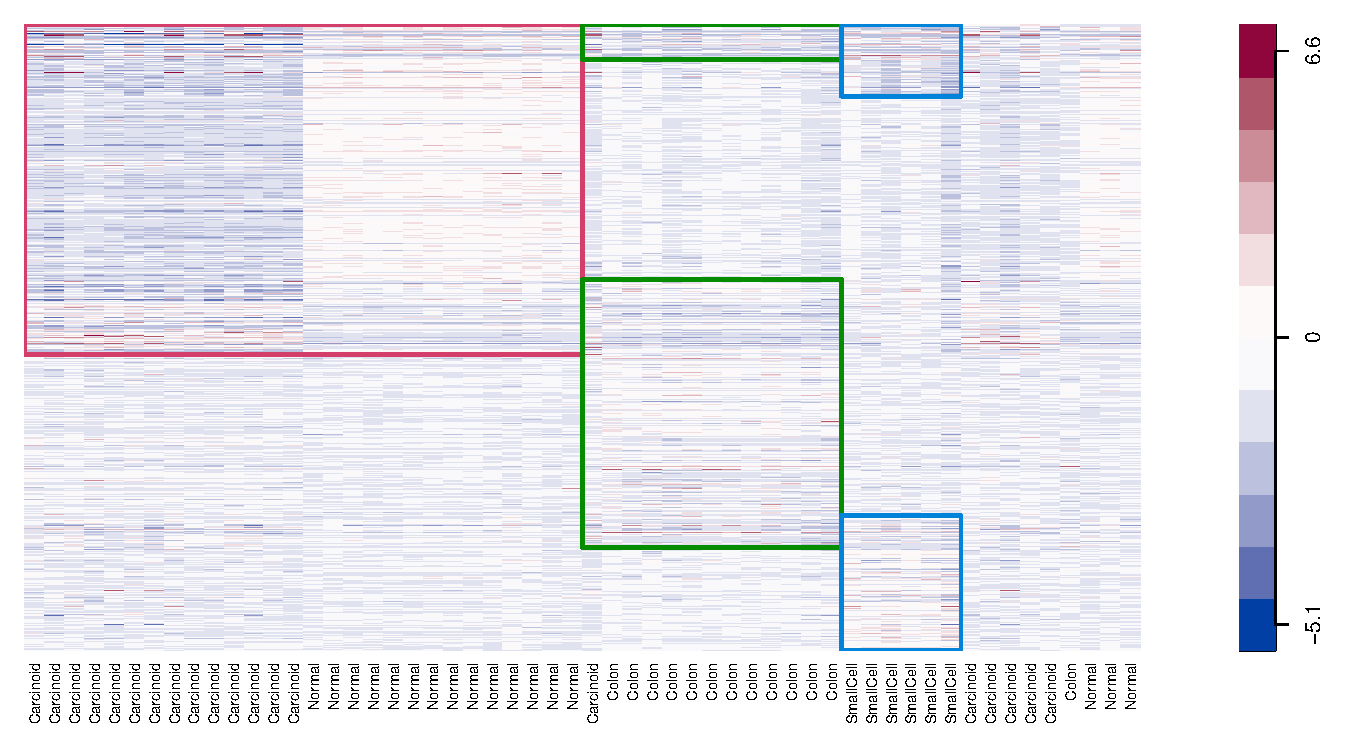
\includegraphics[width=170 mm]{lungheatmap.pdf}
\caption{ Heatmap showing the biclusters identified in the lung cancer data set. Note that the heatmap shows only those genes that have been selected in at least one bicluster. The colored rectangles indicate the genes and samples that correspond to the three biclusters (red corresponds to Bicluster 1, green to Bicluster 2 and blue to Bicluster 3). \label{fig:01} 
}
\end{figure*}

\begin{flushleft}
 \begin{table*}[t]
\processtable{Selection probabilities of lung cancer subclass marker genes \label{Tab:01}}
{\begin{tabular}{lrrrr}\toprule
Gene & \hspace{4 cm} & Bicluster 1 & Bicluster 2 & Bicluster 3 \\[4pt] 
\hline\\[-4pt]
Retinoic acid receptor responder 3 & & 0.99 & 0.00 & 0.00 \\ 
Transforming growth factor, $\beta$ receptor II (70/80kDa) & & 1.00 & 0.00 & 0.86 \\ 
C-type lectin domain family 3, member B (tetranectin) & & 1.00 & 0.74 & 0.68 \\ 
Ficolin (collagen/fibrinogen domain containing) 3 (Hakata antigen) & &1.00 & 0.71 & 0.98 \\ 
v-myc myelocytomatosis viral oncogene homolog & &0.00 & 1.00 & 0.20 \\ 
Integrin, $\alpha$ 6 & &0.00 & 0.93 & 0.00 \\ 
Cyclin-dependent kinase inhibitor 2C (p18) & &0.00 & 0.00 & 0.91 \\ 
Thymosin $\beta$ & &0.00 & 0.15 & 0.98 \\   
\botrule 
\end{tabular}}{}%This is a footnote}
\end{table*}
\end{flushleft}
\begin{center}
\begin{figure*}[t]
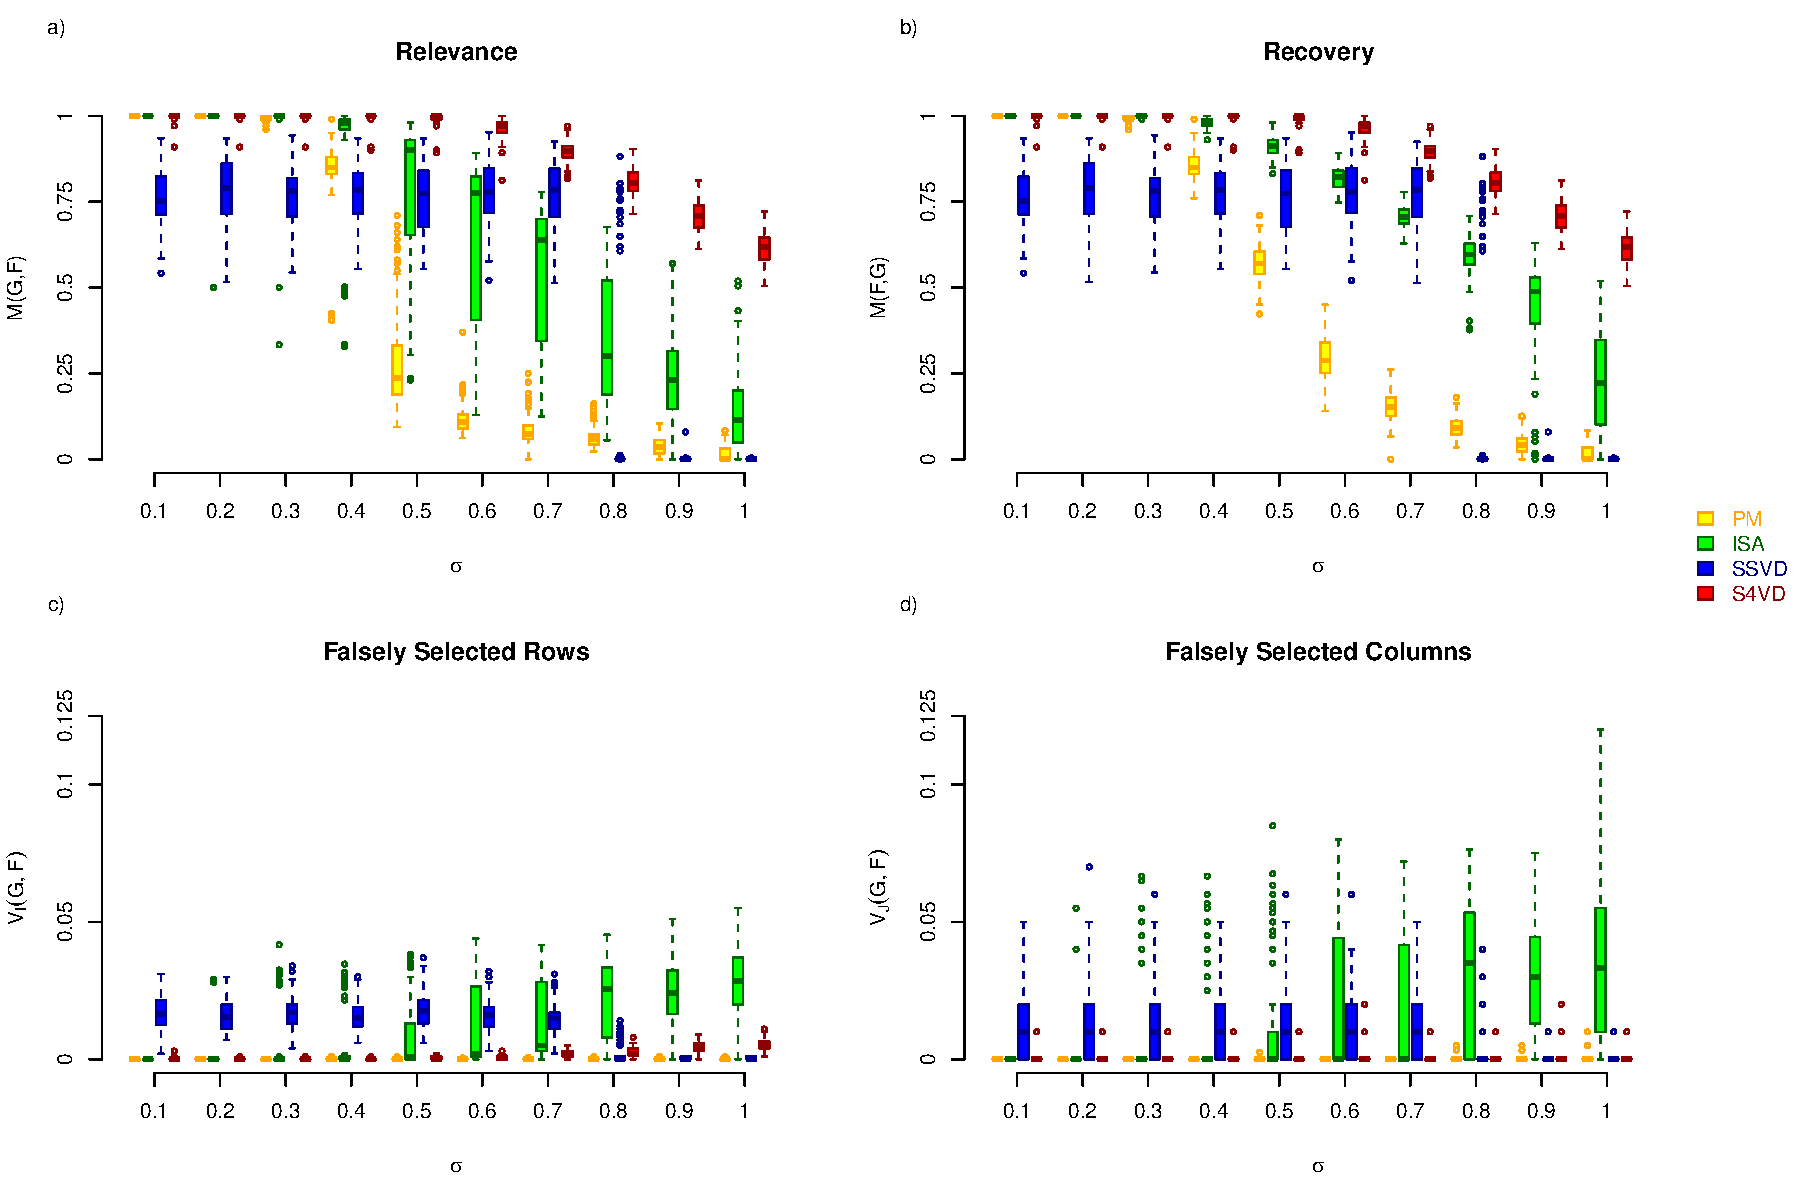
\includegraphics[width=170 mm]{scenario1.pdf}
\caption{ Simulation results of the first scenario. The relevance score $M(G,F)$, recovery score $M(F,G)$ and the average proportions of falsely assigned rows $V_{I}(G,F)$ and columns $V_{J}(G,F)$ are described in the supplementary material. The boxplots show the distribution of these validation indices with respect to the $100$ simulated data sets. $\sigma$ indicates the considered noise level.\label{fig:02} 
}
\end{figure*}
\end{center}
\vspace{-1.5 cm}
\section{Results}
\textcolor{red}{In order to demonstrate that the here proposed S4VD algorithm is able to find biologically relevant biclusters, we applied it to a known lung cancer gene expression data set (Bhattacharyee et al., 2001)\nocite{Bhattacharjee2001}.} Furthermore, to examine the influence of increasing levels of noise regarding the performance of the S4VD algorithm, we performed a simulation study. The S4VD algorithm was compared with the SSVD method, the improved Plaid Model (Turner et al., 2005) and the ISA (Bergmann et al., 2003). The ISA and the Plaid Model are known to be closely related to the SVD.  

\subsection{Evaluation of the lung cancer data set}
Here we analyzed the same subset of the lung cancer gene expression data set (Bhattacharyee et al., 2001) that was used by Lee et al. (2010) to illustrate the SSVD algorithm. This data set contain $56$ samples and gene expression values of $12\,625$ genes measured using the Affymetrix 95av2 GeneChip. The samples comprise $20$ pulmonary carcinoid samples (Carcinoid), $13$ colon cancer metastasis samples (Colon), $17$ normal lung samples (Normal) and $6$ small cell lung carcinoma samples (SmallCell). Lee et al. (2010) applied the SSVD method to this gene expression matrix and decomposed it into the first three sparse SVD-layers. For each of the resulting SVD-layers the \textit{degree of sparsity} was relatively low, e.g. \textcolor{red}{for the three singular vectors that correspond to the samples the number of non-zero coefficients were $55$ for the first two and $47$ for the third.} The singular vectors that correspond to the genes contained $3\,205$, $2\,511$ and $1\,221$ non-zero coefficients. Scatterplots of the sample singular vectors showed a clear grouping of the samples into the different cancer subtypes. In addition, Lee et al. (2010) formed $27$ gene sets according to the sign of the coefficients in the three gene singular vectors. The mean expression profiles of these gene sets showed clear differences between the cancer subtypes. However, despite these results a direct interpretation of each singular vector pair is not possible. 
To obtain SVD-layers with a higher $\textit{degree of sparsity}$ that can be interpreted as single biclusters, we applied the S4VD algorithm controlling a PCER of $0.5$ for falsely selecting coefficients in the sample singular vector and a PCER of $0.01$ for falsely selecting coefficients in the gene singular vector. \textcolor{red}{Furthermore, we did not allow the samples to overlap, e.g. each sample is assigned to only one bicluster.} Therefore, after a sparse SVD-layer is fitted, we exclude the corresponding columns from the data matrix and applied the S4VD algorithm to the resulting submatrix. \textcolor{red}{According to the stopping criterion of the S4VD algorithm} three biclusters have been obtained and are shown in the heatmap in Figure 1. The first bicluster corresponds to a subset of $550$ genes and a subset of $28$ samples including $14$ Normal samples and $14$ Carcinoid samples. The second bicluster comprises $12$ Colon samples and one falsely assigned Carcinoid sample together with a subset of $506$ genes. The third bicluster consists of $6$ SmallCell samples and $344$ genes. All other samples and genes have not been assigned to any bicluster. To illustrate that the selected genes represent genes that are associated with the cancer subtypes we performed a geneset enrichment analysis. Tables of all significantly enriched Gene Ontology (GO) terms ($p<0.01$) as well as a description of the analysis can be found in the supplementary material. 
Bhattacharjee et al. (2001) identified several possible marker genes for the different cancer subtypes. A list of eight of these genes together with the corresponding selection probabilities with respect to the three bicluster are shown in Table 1. \textit{TGF-$\beta$ receptor II}, \textit{tetranectin}, \textit{retinoic acid receptor responder 3} and \textit{ficolin 3} are known to be highly expressed in normal lung tissue compared to carcinoid tissue and thus have high selection probabilities for the first bicluster. This coincides with the GO analysis, e.g. two of the $62$ GO-terms that are significantly enriched by the genes corresponding to the first bicluster are \textit{TGF$\beta$ receptor signaling pathway} (GO:0007179) and \textit{response to retinoic acid} (GO:0032526). \textit{Integrin,$\alpha$6} as well as \textit{v-myc} (\textit{c-myc}) are usually overexpressed in colon cancer. These genes have high selection probabilities with respect to the second bicluster. In addition, among the $61$ significantly enriched GO-terms corresponding to the second bicluster is the term \textit{endothelial cell migration} (GO:0043542) which coincides with the fact that the associated samples correspond to colon cancer metastases. The \textit{cell-cycle inhibitor protein p18} and \textit{thymosin-$\beta$} are markers for small cell carcinomas and show high selection probabilities in the third bicluster. Among the $97$ GO-terms significantly enriched in the third bicluster are many cell cycle associated terms, e.g. \textit{cell division} (GO:0051301), \textit{mitotic spindle organization} (GO:0007052) and \textit{cell cycle checkpoint} (GO:0000075). Furthermore, for the first bicluster as well as for the third bicluster the GO-term \textit{positive regulation of Notch signaling pathway} (GO:0045747) is significantly enriched. Alterations of the Notch signaling cascade are known to be associated with several human cancer types. 
\begin{center}
\begin{figure*}[t]
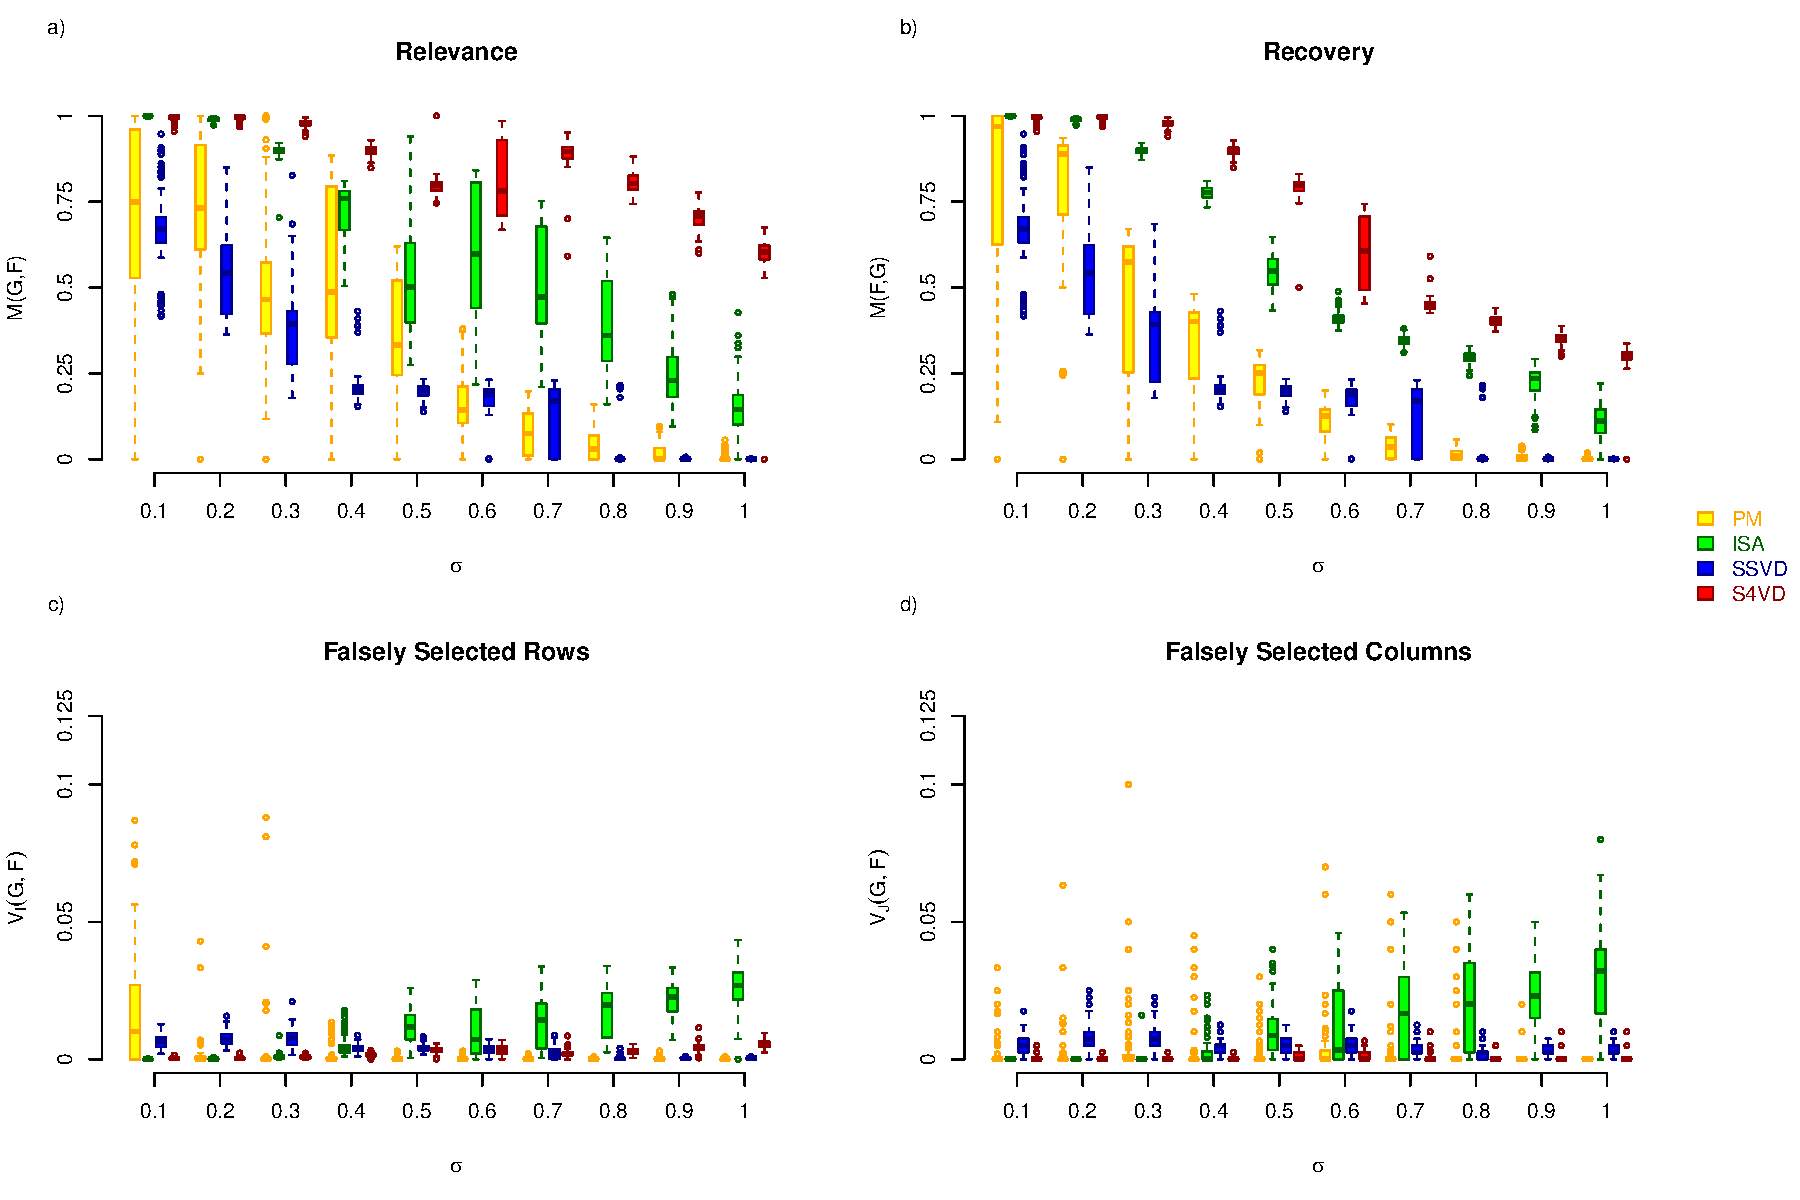
\includegraphics[width=170 mm]{scenario3.pdf}
\caption{ Simulation results of the second scenario. The relevance score $M(G,F)$, recovery score $M(F,G)$ and the average proportions of falsely assigned rows $V_{I}(G,F)$ and columns $V_{J}(G,F)$ are described in the supplementary material. The boxplots show the distribution of these validation indices with respect to the $100$ simulated data sets. $\sigma$ indicates the considered noise level. \label{fig:03} 
}
\end{figure*}
\end{center}

\subsection{Simulation study}
In the first part of the simulations we generated $100$ artificial data matrices comprising $p=1000$ genes and $n=100$ samples, where each entry of the data matrix is set to $0$. In each dataset we randomly assigned $100$ genes and $10$ samples to a bicluster that shows constant upregulated gene expression represented by a value of $1$ in the data matrix. Normally distributed noise $\text{N}(0,\sigma)$ was added to each entry of the data matrix. We examined different noise levels in the range of $\sigma=(0,0.1,\cdots,1)$. In the second part of the simulation study $100$ data matrices of the same dimension were generated. This time four biclusters were included where each consists of $100$ genes and $10$ samples. Constant up- and down-regulation was represented by values of 1,-1,0.5 and -0.5. For both scenarios the performance of the S4VD algorithm was examined in comparison to the original SSVD algorithm, the improved Plaid Model (PM; Turner et al., 2005) and the ISA (Bergmann et al., 2003). Since the SSVD algorithm does not include a stopping criterion, we considered only the first SVD-layer as result in the first scenario and the first four SVD-layers as the biclustering result in the second scenario. The clustering results were validated by application of an external validation index based on the Jaccard coefficient. In addition, the stability of the clustering results was assessed through the average proportion of falsely selected rows and columns. Details on the validation indices, the remaining biclustering algorithms and their relation to the SVD are provided in the supplementary material. 
\subsubsection{Scenario 1}
The simulation results of the first scenario are shown in Figure 2. For low noise levels up to $\sigma=0.3$ all biclustering algorithms except the SSVD show an almost perfect performance with relevance and recovery scores mostly equal to one and no falsely selected rows and columns. 
For noise levels of $0.1$ to $0.7$ all biclusters proposed by the SSVD algorithm are too large and on average a proportion around $0.015$ of the rows and $0.012$ of the columns are falsely assigned. This results in relevance and recovery scores around $0.8$. In case of larger noise levels the SSVD algorithm often fails to converge and thus the relevance scores and the number falsely assigned rows and columns approach zero. 
For noise levels above $0.3$ the first bicluster detected by the Plaid Model usually consists of a strict subset of those rows and columns that belong to the true artificial bicluster in the data. Thus the performance of the Plaid Model regarding the relevance and the recovery decreases with noise. 
Furthermore, the algorithm starts to fit the noise and proposes a number of further small biclusters. This explains why the relevance score is inferior compared to the recovery score. Most of these small biclusters correspond to parts of the true artificial bicluster and hence the proportions of falsely assigned rows and columns are close to zero. Beginning with a noise level of $0.5$ the ISA proposes an increasing number of biclusters of which only one shows a strong agreement with the true bicluster. Even after applying the additional filtering functions available in the \textit{isa2} R-package (Csardi et al., 2010) some nonsense biclusters remain. Thus both scores start to decrease with noise but are superior to the Plaid Model. The number of falsely assigned rows and columns increases with the noise level indicating that some of the detected biclusters correspond to fitted noise. Regardless of the noise level the S4VD algorithm always detects a single bicluster that agrees with the true bicluster. For noise levels above $0.6$ the proposed bicluster becomes smaller and represents only a part of the true bicluster. Therefore both scores start to decrease with noise but are superior to that of all other biclustering methods considered in the simulation study. %Due to the stability selection the S4VD algorithm rarely assigns false rows and columns to the proposed bicluster and does not detect any additional nonsense clusters. Thus the average proportions of falsely assigned rows and columns are almost zero for all noise levels. 

\subsubsection{Scenario 2}
The results of the second part of the simulation study are shown in Figure 3. For noise levels below $0.3$ the ISA and the S4VD showed relevance and recovery scores around $1$ and the according average proportions of falsely assigned objects are near zero. This indicates that both algorithms are able to correctly detect all of the four artificial biclusters present in the data. 
The Plaid Model algorithm in some cases perfectly revealed the hidden structure, but in other situations depending on the randomly chosen starting values and the noise level the algorithm falsely assigns rows and columns to the biclusters. The stopping criterion of the algorithm depends on a permutation test that can fail to reject unimportant biclusters that correspond to noise. On the other hand for higher noise levels the permutation test also tends to reject biclusters early in the fitting process so that only three or less biclusters are detected. Thus the resulting relevance and recovery scores are highly variable and decrease with noise.
Regarding low noise levels, the SSVD algorithm mostly identifies the correct biclusters but usually falsely assigns some additional rows and columns. This behavior maintains for higher noise levels, but additionally the number of correctly identified biclusters becomes less. \textcolor{red}{For noise levels above 0.7 both the SSVD algorithm and the Plaid Model mostly do not detect any of the artificial biclusters and hence the average proportions of falsely assigned rows and columns approach zero.}
The performance of the ISA decreases due to an increasing number of identified irrelevant biclusters, starting with noise levels above $0.2$. For noise level $0.5$ the medians of both similarity scores are approximately $0.5$ and the relevance scores show a high variability. For noise levels above $0.5$ the two embedded biclusters generated to have a constant up- and down-regulation of $0.5$ and $-0.5$ are masked by noise, and hence, the ISA as well as the S4VD algorithm tend to miss these clusters. This results in a slight increase of their relevance scores while the recovery scores decrease. Moreover, the relevance scores for both algorithms show a high variability at noise level \textcolor{red}{$0.6$}. \textcolor{red}{In summary, the S4VD algorithm outperforms all other biclustering algorithms considered in the simulation study regarding the relevance and the recovery of the artificial biclusters for all simulation scenarios. Furthermore, due to the stability selection the S4VD algorithm rarely assigns false rows and columns to the proposed bicluster and does not detect any additional nonsense clusters. Thus for all simulation scenarios the average proportions of falsely assigned rows and columns are close to zero. } 

\section{Discussion and Conclusion}
In this paper we propose a new biclustering algorithm which combines the SSVD algorithm suggested by Lee et al. (2010) with the stability selection of Meinshausen and B\"uhlmann (2010). In brief, the model selection based parameter tuning of the penalized regression models of the SSVD algorithm is replaced by a subsampling based variable selection that controls Type I error rates. The S4VD approach here presented allows to control the \textit{degree of sparsity} of the resulting SVD-layers by choosing desired Type I error levels. The stability selection estimates the selection probabilities of the rows and columns to belong to a bicluster. %These selection probabilities are an additional information supporting the interpretation of the clustering results. 
Depending on the chosen Type I error levels the results are robust biclusters represented by rows and columns that have high selection probabilities. If the noise level is getting too high the stopping criterion leads to an interruption of the S4VD algorithm preventing from fitting additional SVD-layers that correspond to noise. %In addition, due to the higher \textit{degree of sparsity} of the resulting SVD-layers, a biological interpretation is more straightforward compared to the SSVD algorithm. 
So far, the S4VD method is the only biclustering approach that takes the cluster stability regarding perturbations of the data into account. 
We applied the S4VD algorithm to evaluate a lung cancer microarray data set and showed that the resulting biclusters represent tumor subclasses together with coregulated genes. \textcolor{red}{Marker genes for the different tumor subclasses showed high selection probabilities in the respective biclusters. In addition, a gene set enrichment analysis revealed that the genes associated with identified biclusters belong to significantly enriched cancer related Gene Ontology terms. In a simulation study the S4VD algorithm was compared with the SSVD algorithm, the improved Plaid Model (Turner et al., 2005) and the ISA (Bergmann, 2003). The S4VD algorithm showed the best performance regarding the recovery of biclusters and was more robust to noisy data compared to the other methods.} 
\textcolor{red}{The subsampling steps of the stability selection make the S4VD algorithm computationally very demanding. However, an improvement that strongly reduces the computation time is presented in the supplementary material.} 

\nocite{Alexa2006}
\nocite{Csardi2010}
\nocite{biclust}

%%%%%%%%%%%%%%%%%%%%%%%%%%%%%%%%%%%%%%%%%%%%%%%%%%%%%%%%%%%%%%%%%%%%%%%%%%%%%%%%%%%%%
%
%     please remove the " % " symbol from \centerline{\includegraphics{fig01.eps}}
%     as it may ignore the figures.
%
%%%%%%%%%%%%%%%%%%%%%%%%%%%%%%%%%%%%%%%%%%%%%%%%%%%%%%%%%%%%%%%%%%%%%%%%%%%%%%%%%%%%%%

\bibliographystyle{natbib}

\bibliography{document.bib}

\end{document}
 